% Options for packages loaded elsewhere
\PassOptionsToPackage{unicode}{hyperref}
\PassOptionsToPackage{hyphens}{url}
%
\documentclass[
]{article}
\title{Crab Species ID Guide}
\author{Gena Desjardin}
\date{10/17/2021}

\usepackage{amsmath,amssymb}
\usepackage{lmodern}
\usepackage{iftex}
\ifPDFTeX
  \usepackage[T1]{fontenc}
  \usepackage[utf8]{inputenc}
  \usepackage{textcomp} % provide euro and other symbols
\else % if luatex or xetex
  \usepackage{unicode-math}
  \defaultfontfeatures{Scale=MatchLowercase}
  \defaultfontfeatures[\rmfamily]{Ligatures=TeX,Scale=1}
\fi
% Use upquote if available, for straight quotes in verbatim environments
\IfFileExists{upquote.sty}{\usepackage{upquote}}{}
\IfFileExists{microtype.sty}{% use microtype if available
  \usepackage[]{microtype}
  \UseMicrotypeSet[protrusion]{basicmath} % disable protrusion for tt fonts
}{}
\makeatletter
\@ifundefined{KOMAClassName}{% if non-KOMA class
  \IfFileExists{parskip.sty}{%
    \usepackage{parskip}
  }{% else
    \setlength{\parindent}{0pt}
    \setlength{\parskip}{6pt plus 2pt minus 1pt}}
}{% if KOMA class
  \KOMAoptions{parskip=half}}
\makeatother
\usepackage{xcolor}
\IfFileExists{xurl.sty}{\usepackage{xurl}}{} % add URL line breaks if available
\IfFileExists{bookmark.sty}{\usepackage{bookmark}}{\usepackage{hyperref}}
\hypersetup{
  pdftitle={Crab Species ID Guide},
  pdfauthor={Gena Desjardin},
  hidelinks,
  pdfcreator={LaTeX via pandoc}}
\urlstyle{same} % disable monospaced font for URLs
\usepackage[margin=1in]{geometry}
\usepackage{graphicx}
\makeatletter
\def\maxwidth{\ifdim\Gin@nat@width>\linewidth\linewidth\else\Gin@nat@width\fi}
\def\maxheight{\ifdim\Gin@nat@height>\textheight\textheight\else\Gin@nat@height\fi}
\makeatother
% Scale images if necessary, so that they will not overflow the page
% margins by default, and it is still possible to overwrite the defaults
% using explicit options in \includegraphics[width, height, ...]{}
\setkeys{Gin}{width=\maxwidth,height=\maxheight,keepaspectratio}
% Set default figure placement to htbp
\makeatletter
\def\fps@figure{htbp}
\makeatother
\setlength{\emergencystretch}{3em} % prevent overfull lines
\providecommand{\tightlist}{%
  \setlength{\itemsep}{0pt}\setlength{\parskip}{0pt}}
\setcounter{secnumdepth}{-\maxdimen} % remove section numbering
\ifLuaTeX
  \usepackage{selnolig}  % disable illegal ligatures
\fi

\begin{document}
\maketitle

\newpage

\hypertarget{pagurus-hirsutiusculus-hairy-hermit-crab}{%
\section{\texorpdfstring{\emph{Pagurus hirsutiusculus} (Hairy Hermit
Crab)}{Pagurus hirsutiusculus (Hairy Hermit Crab)}}\label{pagurus-hirsutiusculus-hairy-hermit-crab}}

\hypertarget{description}{%
\subsection{Description}\label{description}}

Each organism can be black, brown or dark green (Meschkat et al., 2014).
Shell shape can vary but shape of the actual body is fairly consistent
with the shield of the carapace (most cranial part of the back of the
crab) being less long than it is wide (Jensen, 2014). Body size can
reach 2 cm (Meschkat et al., 2014). The hairy hermit crab has hairs
along its body (Meschkat et al., 2014). However, the amount of hairs can
vary from one individual to another (Jensen, 2014). On its walking legs,
these crabs have a white band by the last joint (Meschkat et al., 2014).
More white bands may be present if the individual is young (Jensen,
2014). Also, their walking legs often have at most two blue dots on each
leg though these may be more difficult to see (Meschkat et al., 2014).
Small light rings encircle their antennae (Meschkat et al., 2014).

\textbf{Species lookalike}

It possesses one lookalike species: \emph{Pagurus carinus} (the
greenmark hermit crab) (Meschkat et al., 2014). However, this crab lacks
rings on the antennae, possesses spiny claws and has a carapace that
only reaches 1 cm which is half the size as that of the hairy hermit
crab (Harbo, 2011).

\textbf{Range, Habitat, Diet, Foraging Mode and Reproduction}

These crabs can be found between California (Monterey) and Alaska
(Pribilof Islands) (Harbo, 2011). They live in protected areas including
the intertidal zone in tidepools protected by algae (Meschkat et al.,
2014; Harbo, 2011). On the rare occasion, they may be found up to 110m
subtidally (Harbo, 2011). These crabs are detritivores, thus they eat
dead organisms but will eat other live animals if available, thus making
them consumers as well (Cowles, 2005b). They actively search for food by
walking around (Jensen, 2014). They undergo sexual reproduction and are
oviparous meaning they lay eggs (Kornienko, 2020).

\newpage

\hypertarget{figures}{%
\subsection{Figures}\label{figures}}

\begin{figure}

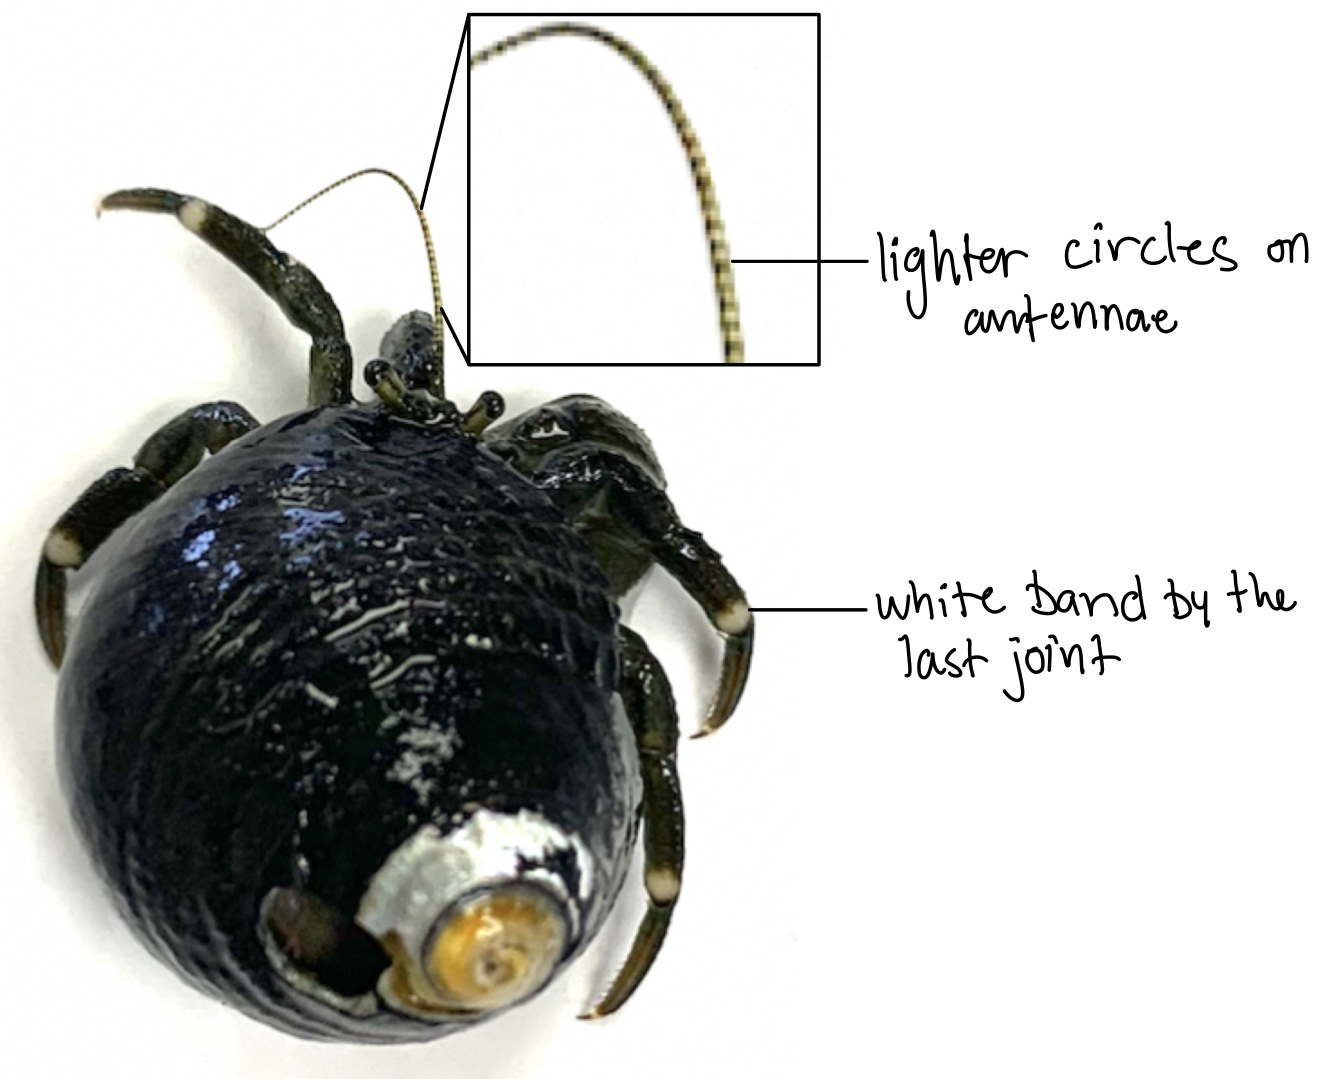
\includegraphics[width=0.5\linewidth,height=0.3\textheight]{C:/Users/bmsuser/Github/species-id-guide-genagardens/images/hairy-hermit-full-labeled} \hfill{}

\caption{Photo of a black/dark green $\textit{Pagurus hirsutiusculus}$ including labeled diagnostic features}\label{fig:hairy-hermit}
\end{figure}

\begin{figure}

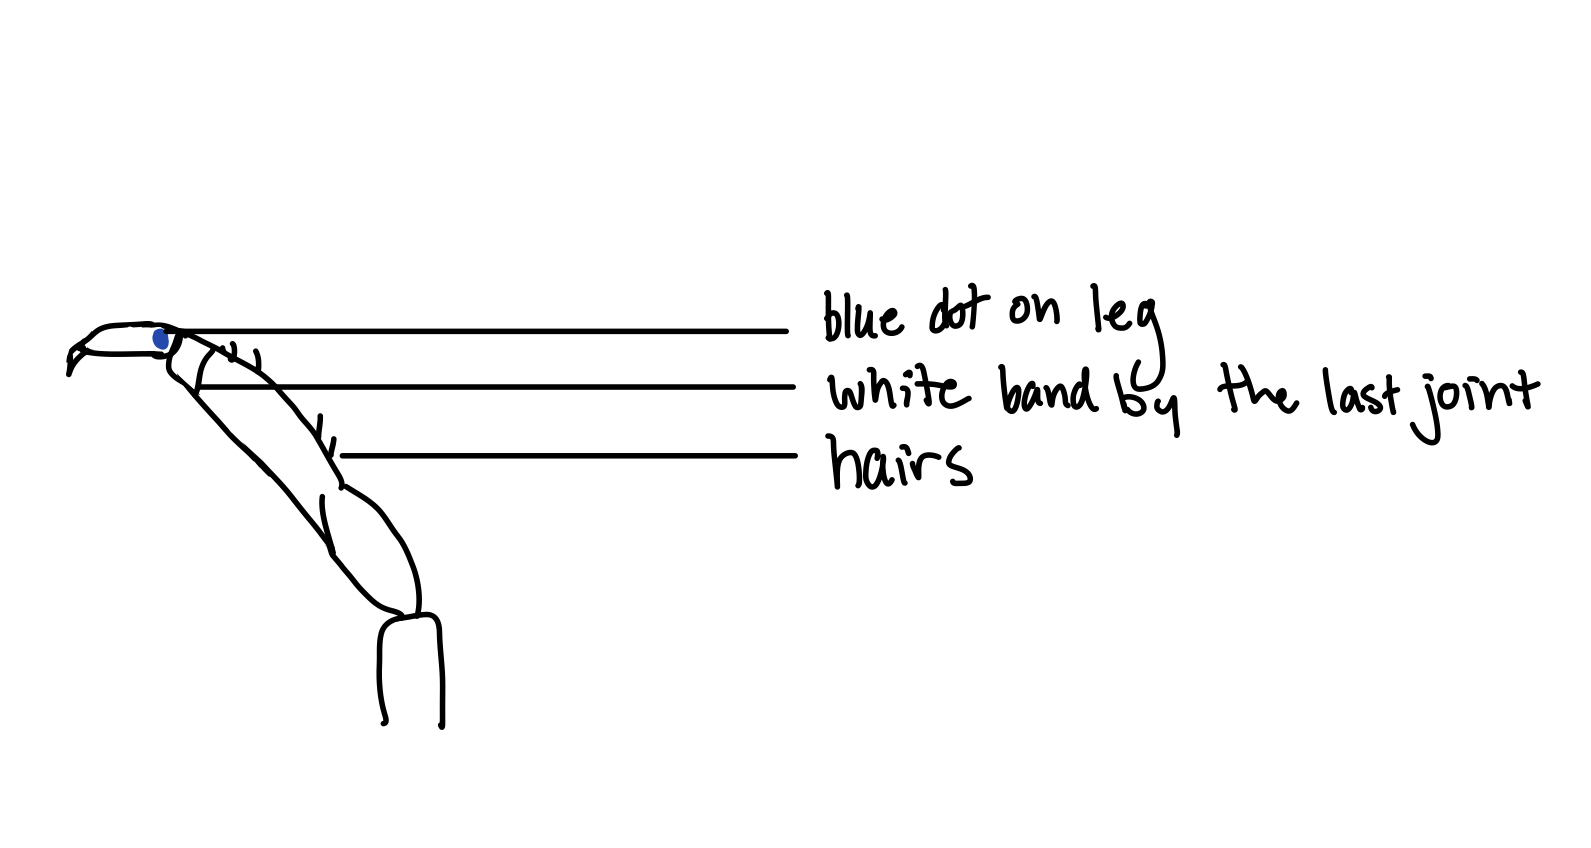
\includegraphics[width=0.5\linewidth,height=0.3\textheight]{C:/Users/bmsuser/Github/species-id-guide-genagardens/images/hairy-hermit-leg-drawing} \hfill{}

\caption{Drawing of the leg of $\textit{Pagurus hirsutiusculus}$ including labeled diagnostic features}\label{fig:hairy-hermit-leg}
\end{figure}

\begin{figure}

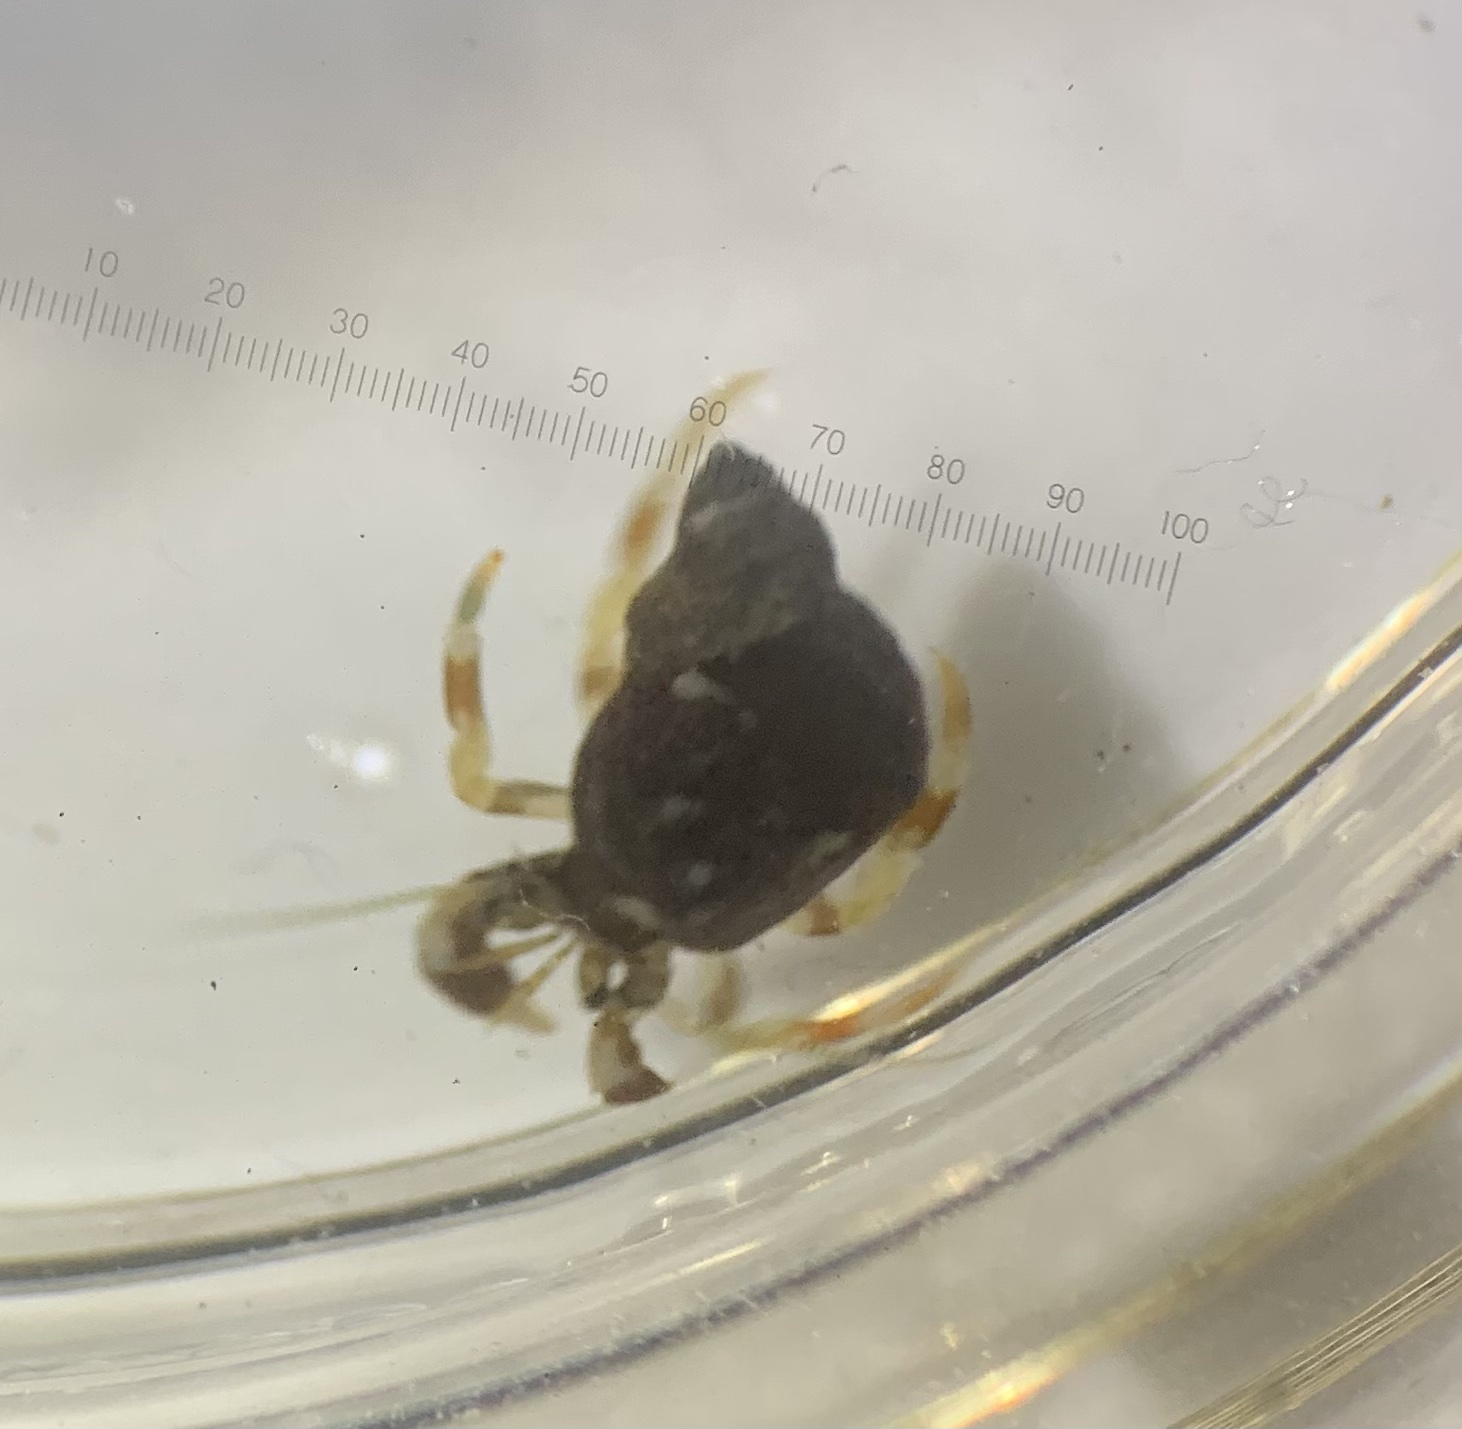
\includegraphics[width=0.5\linewidth,height=0.3\textheight]{C:/Users/bmsuser/Github/species-id-guide-genagardens/images/baby-hairy-hermit} \hfill{}

\caption{A brown juvenile $\textit{Pagurus hirsutiusculus}$ under a dissecting microscope, demonstrating the extra white bandings}\label{fig:hairy-hermit-juvenile}
\end{figure}

\begin{figure}

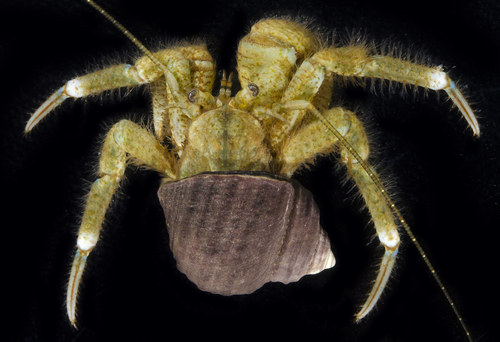
\includegraphics[width=0.5\linewidth,height=0.3\textheight]{C:/Users/bmsuser/Github/species-id-guide-genagardens/images/iNaturalist copy} \hfill{}

\caption{A green/brown $\textit{Pagurus hirsutiusculus}$ demonstrating a substantial amount of hairs (Photo Credits: Hakai Institute, iNaturalist)}\label{fig:hair-hermit-very-hairy}
\end{figure}

\newpage

\hypertarget{questions}{%
\subsection{Questions}\label{questions}}

\begin{enumerate}
\def\labelenumi{\arabic{enumi}.}
\tightlist
\item
  Are there hairs on the body?
\item
  Are there white bands around the last joints of the first two legs?
\item
  Are there rings circling around the antennae?
\end{enumerate}

\newpage

\hypertarget{pagurus-granosimanus-grainyhand-hermit-crab}{%
\section{\texorpdfstring{\emph{Pagurus granosimanus} (Grainyhand Hermit
Crab)}{Pagurus granosimanus (Grainyhand Hermit Crab)}}\label{pagurus-granosimanus-grainyhand-hermit-crab}}

\hypertarget{description-1}{%
\subsection{Description}\label{description-1}}

The grainyhand hermit's has an olive-green carapace and claws that are
dotted with white or blue granules (Fretwell, 2015). It has distinct
solid orange antennae and prefers shells that it can completely withdraw
into, often looking disproportionately large for its body (Fretwell,
2015). Shells it typically inhabits include black turban snails
(\emph{Tegula funebralis}), dire whelks (\emph{Lirabuccinum dirum}), and
frilled dogwinkle (\emph{Nucella lamellosa}) (Fretwell, 2015). They can
grow up to 2cm and select different shells as they continue to grow
(Jensen, 1995).

\textbf{Species lookalike}

Some similar looking species such as the Bering hermit, (\emph{Pagurus
beringanus}) have red dots and bands on the legs; the hairy hermit
(\emph{Pagurus hirsutiusculus}) is covered in small hairs and has no
dots; the Maroon hermit (\emph{Pagurus hemphilli}) is dark red with
white, yellow, or blue dots and light coloured leg tips; lastly, the
blueband hermit has irregular, but bright blue banding near the ends of
walking legs and its carapace is striped (Cowles, 2005a; Jensen, 1995).

\textbf{Range, Habitat, Diet, Foraging Mode and Reproduction}

\emph{P. granosimanus} is common in both mid and low intertidals
tidepools or under rocks on protected rocky shores (Jensen, 1995). It
can also be found in larger groups on shallow sand bottoms (Jensen,
1995). The deepest recorded finding was at 36 m in the subtidal (Jensen,
1995). \emph{P. granosimanus} is usually found lower on beaches than the
hairy hermit \emph{P. hirsutiusculus} and higher than the Bering hermit
\emph{P. beringanus} (Jensen, 1995). The grainyhand hermit can be found
from northern Alaska to northern Mexico (Fretwell, 2015).

Like other members of Paguridae, \emph{P. granosimanus} may feed on a
range of foods and will sort through sediment for organic material with
their mouthparts (Jensen, 1995). However, \emph{P. granosimanus} can
also filter feed with its maxillipeds, scavenge, and even prey on
smaller organisms (Jensen, 1995). Its right claw is notably larger than
its left, which may allow for a wider range of potential foods (Jensen,
1995).

Females of many decapod species can only mate while soft shelled
(Jensen, 1995). Females approaching their molting phase are thought to
release pheromones to attract males (Jensen, 1995). As noted of the
different claw sizes for feeding, larger claw size differences are seen
in males. This indicates that claw sizing may play an important role in
mate selection as Paguridae males will drag around females awaiting
their molting phase to mate (Jensen, 1995). These males will use their
smaller claw to hold onto the female while warding off rival males with
their larger claw (Jensen, 1995). When the female molts the male will
reposition for copulation to occur and will often continue the embrace
afterwards (Jensen, 1995). Females will brood their eggs in their
pleopods, a set of their hind legs (Jensen, 1995). They will pick out
dead eggs and even aerate them (Jensen, 1995). The female releases the
eggs once ready to hatch (Jensen, 1995).

\newpage

\begin{figure}

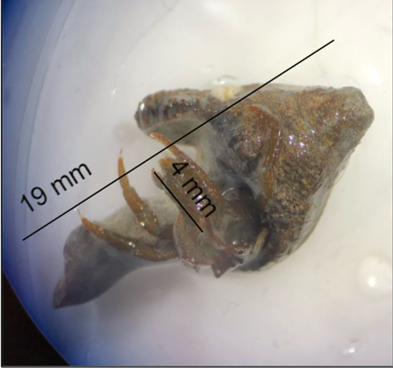
\includegraphics[width=0.5\linewidth,height=0.3\textheight]{C:/Users/bmsuser/Github/species-id-guide-genagardens/images/Grainyhand_size} \hfill{}

\caption{Grainyhand hermit crab size.}\label{fig:Grainyhand_size}
\end{figure}

\begin{figure}

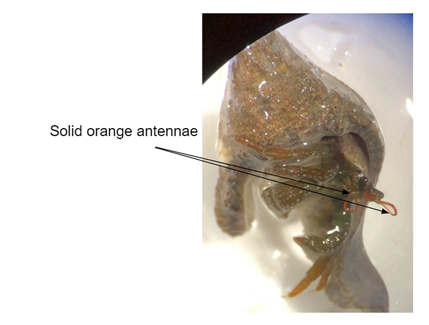
\includegraphics[width=0.5\linewidth,height=0.3\textheight]{C:/Users/bmsuser/Github/species-id-guide-genagardens/images/Grainyhand_antennae} \hfill{}

\caption{Grainyhand hermit crab antennae.}\label{fig:Grainyhand_antennae}
\end{figure}

\begin{figure}

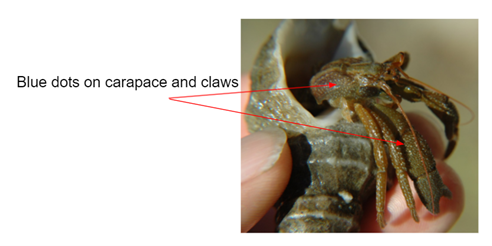
\includegraphics[width=0.5\linewidth,height=0.3\textheight]{C:/Users/bmsuser/Github/species-id-guide-genagardens/images/Grainyhand_blue_dots} \hfill{}

\caption{Grainyhand hermit crab blue dots.}\label{fig:Grainyhand_blue_dots}
\end{figure}
\begin{figure}

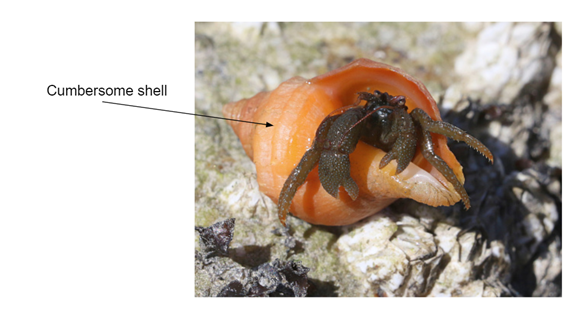
\includegraphics[width=0.5\linewidth,height=0.3\textheight]{C:/Users/bmsuser/Github/species-id-guide-genagardens/images/Grainyhand_cumbersome_shell} \hfill{}

\caption{Grainyhand hermit crab shell, (photo credits: randimal, 2015).}\label{fig:Grainyhand_cumbersome_shell}
\end{figure}
\newpage

\hypertarget{questions-1}{%
\subsection{Questions:}\label{questions-1}}

1.Is it dotted with white or blue granules?\\
2.Are the antennae solid (unbanded) and orange?\\
3.Does the shell look disproportionately large and can it withdraw
completely into its shell?

\newpage

\hypertarget{petrolisthes-cinctipes-flat-porcelain-crab}{%
\section{\texorpdfstring{\emph{Petrolisthes cinctipes} (Flat Porcelain
Crab)}{Petrolisthes cinctipes (Flat Porcelain Crab)}}\label{petrolisthes-cinctipes-flat-porcelain-crab}}

\hypertarget{description-2}{%
\subsection{Description}\label{description-2}}

The flat porcelain crab, \emph{Petrolisthes cinctipes}, has lots of
colour variation - it can be light brown, reddish brown, dark brown,
brown with a blue tinge or a vibrant blue colour (Jensen, 1995). It is
also variable in size, with carapace width reaching up to 24 mm. This
small intertidal shore crab has orange-red mouth parts and claw spots,
as well as distinctly red antennae. The walking legs of \emph{P.
cinctipes} have small uncalcified windows along the joints. They
frequently have one claw with a gap between the pincers (the purpose of
which is unknown) and small round punctures along the claws from
fighting with its rock-mates for space (Jensen, 1995).

\textbf{Species lookalike}

Easily mistaken for the flattop porcelain crab, \emph{P. cabrilloi},
these two species can be distinguished from one another through two key
characteristics (Jensen, 2014). Firstly, \emph{P. cinctipes} has
hairless or limited hair on its walking legs and the carapus of its
claws, while \emph{P. cabrilloi} has distinctly hairy claws and legs.
Secondly, the flattop is more common in sheltered areas, while the flat
porcelain tends to avoid the fine sedimentation found in those areas. As
such, \emph{P. cinctipes} tends to be found in more rocky, wave-exposed
areas (Jensen, 2014).

\textbf{Range, Habitat, Diet, Foraging Mode and Reproduction}

Flat porcelain crabs are found throughout the Pacific Northwest. Their
range spans from Porcher Island, British Columbia to Santa Barbara,
California (Fretwell, K., 2014). They live under rocks in the upper and
middle intertidal, but generally avoid fine sediment. Due to this
aversion to sand, they are primarily restricted to upper levels of
beaches. Furthermore, they are often very abundant in California sea
mussel beds (Fretwell, K., 2014).

\emph{P. cinctipes} is a fairly omnivorous species (Cowles, 2006). They
feed most frequently on plankton and detritus suspended in the water
column. Flat porcelain crabs catch these small particles by waving their
feather-like mouthparts, called maxillipeds and found on the underside
of their head, through the water. \emph{P. cinctipes} also occasionally
eat macroalgae (seaweed) and dead animal tissue (Cowles, 2006).

\emph{P. cinctipes} sexually reproduces continuously in California and
in the spring in Puget Sound (Cowles, 2006). When ready to hatch, a
fertilized egg clutch is laid by the female and is initially bright red,
before fading to brownish red. A single egg clutch is often fertilized
by multiple males, which is likely a reproductive advantage as it
facilitates genetic diversity (Yockachonis, T., 2020).

\newpage

\hypertarget{figures-1}{%
\subsection{Figures}\label{figures-1}}

\begin{figure}

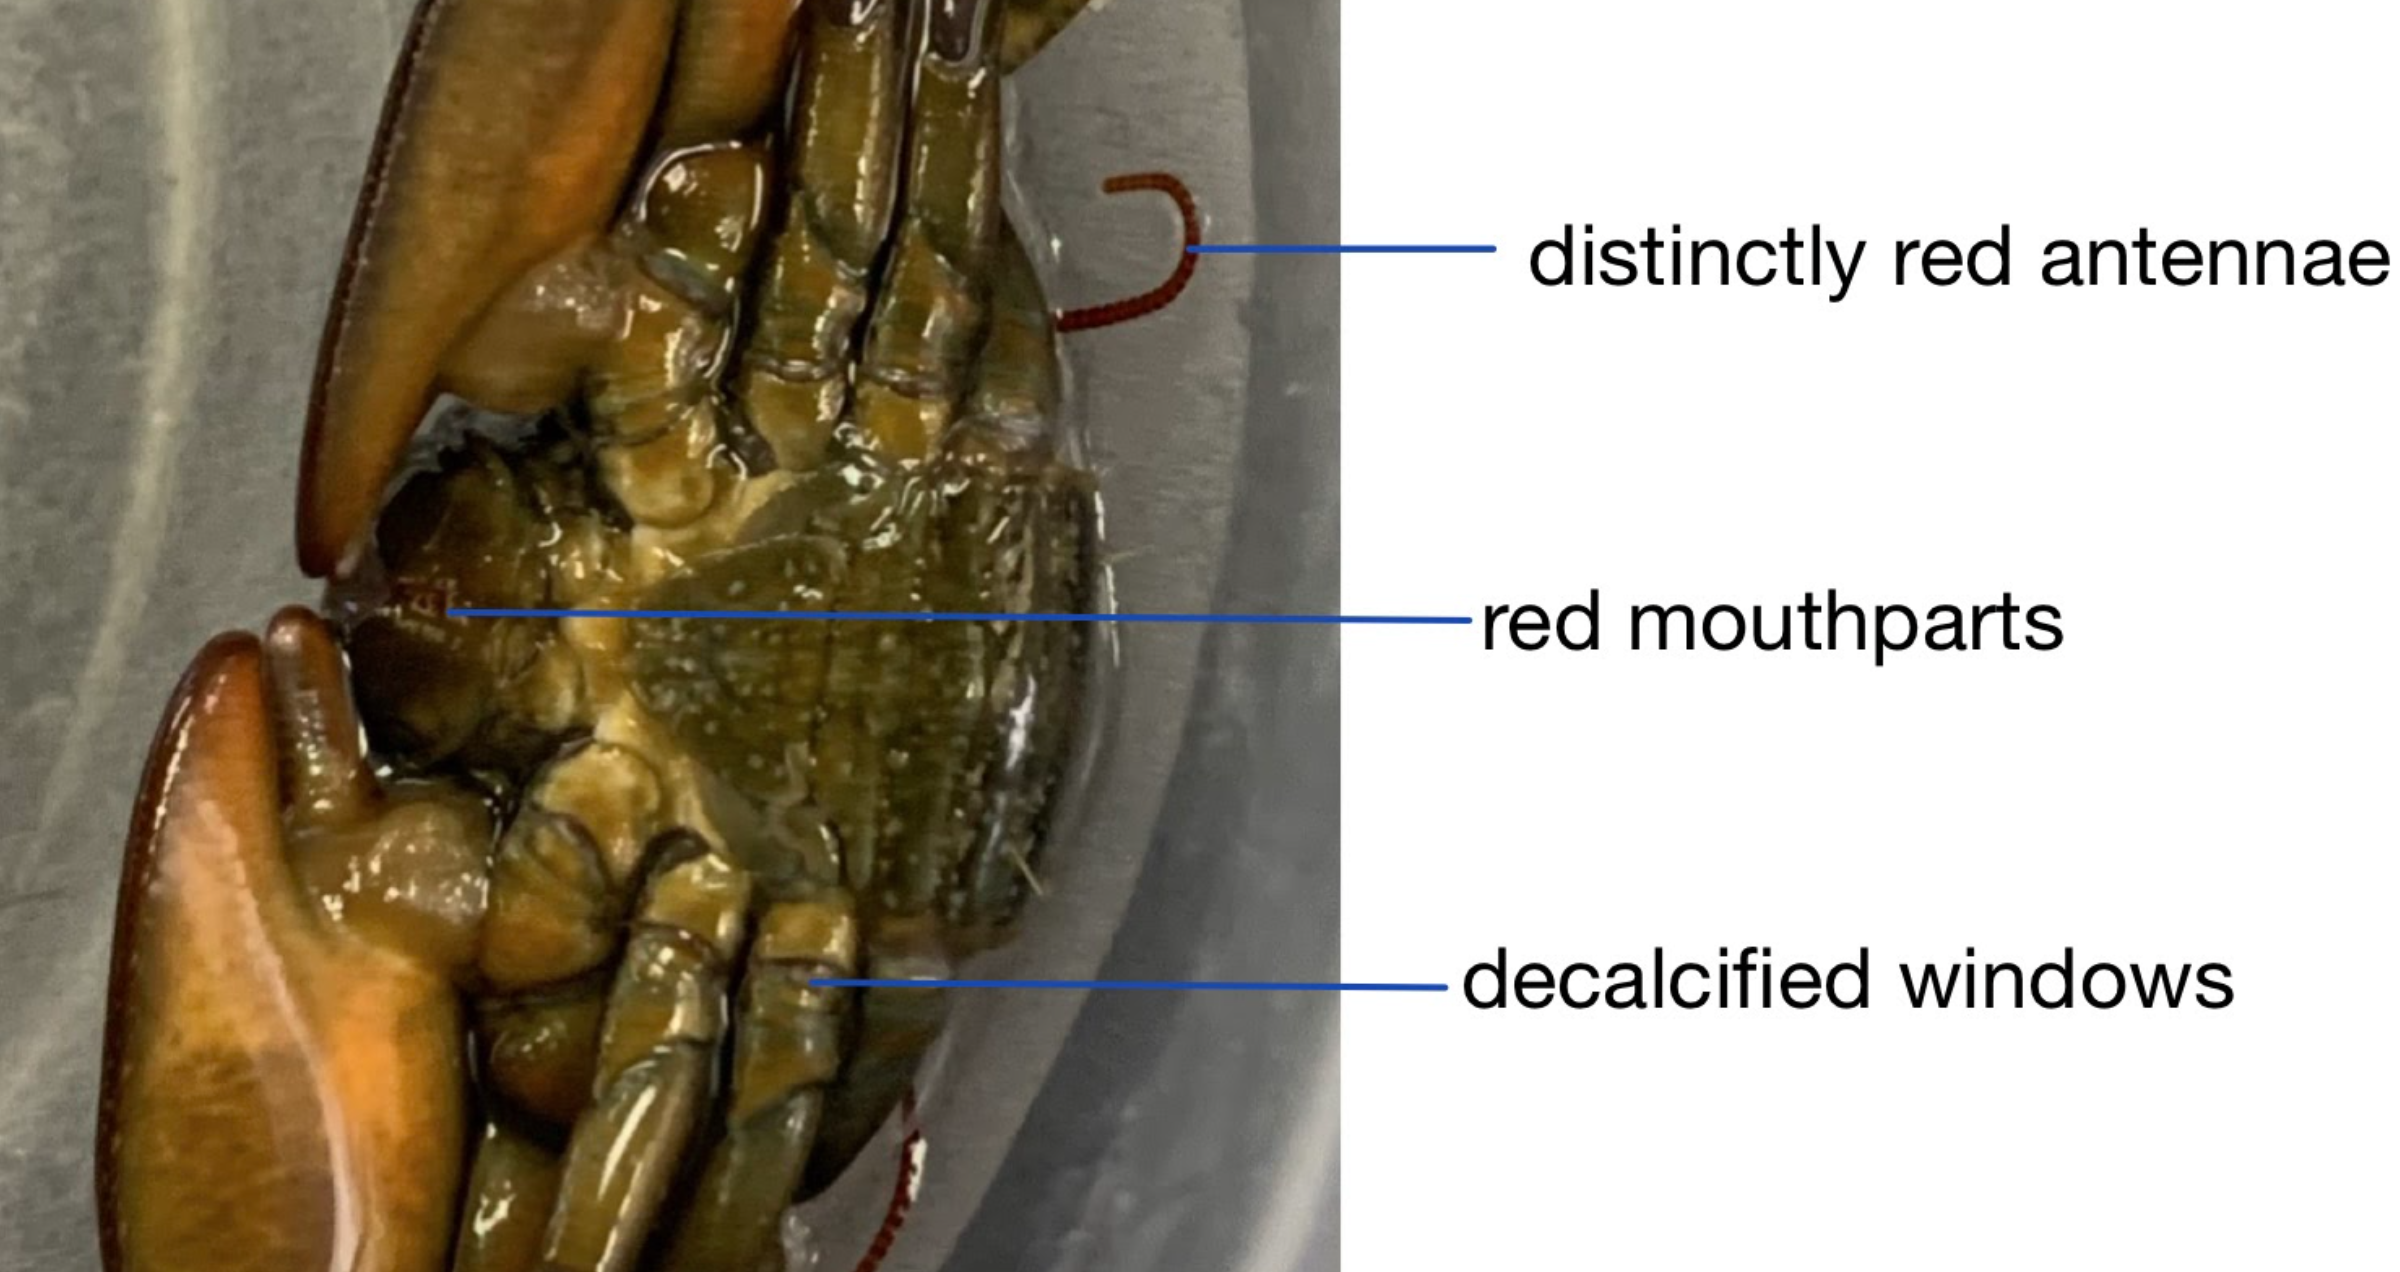
\includegraphics[width=0.5\linewidth,height=0.3\textheight]{C:/Users/bmsuser/Github/species-id-guide-genagardens/images/porcelain.base} \hfill{}

\caption{This is the underside of the flat porcelain crab.}\label{fig:porcelain.base}
\end{figure}

\begin{figure}

\includegraphics[width=0.5\linewidth,height=0.3\textheight]{C:/Users/bmsuser/Github/species-id-guide-genagardens/images/porcelain.blue} \hfill{}

\caption{A blue flat porcelain crab to show morphological diversity (photo credits: Jamie Kish, iNaturalist).}\label{fig:blue.porcelain}
\end{figure}

\begin{figure}

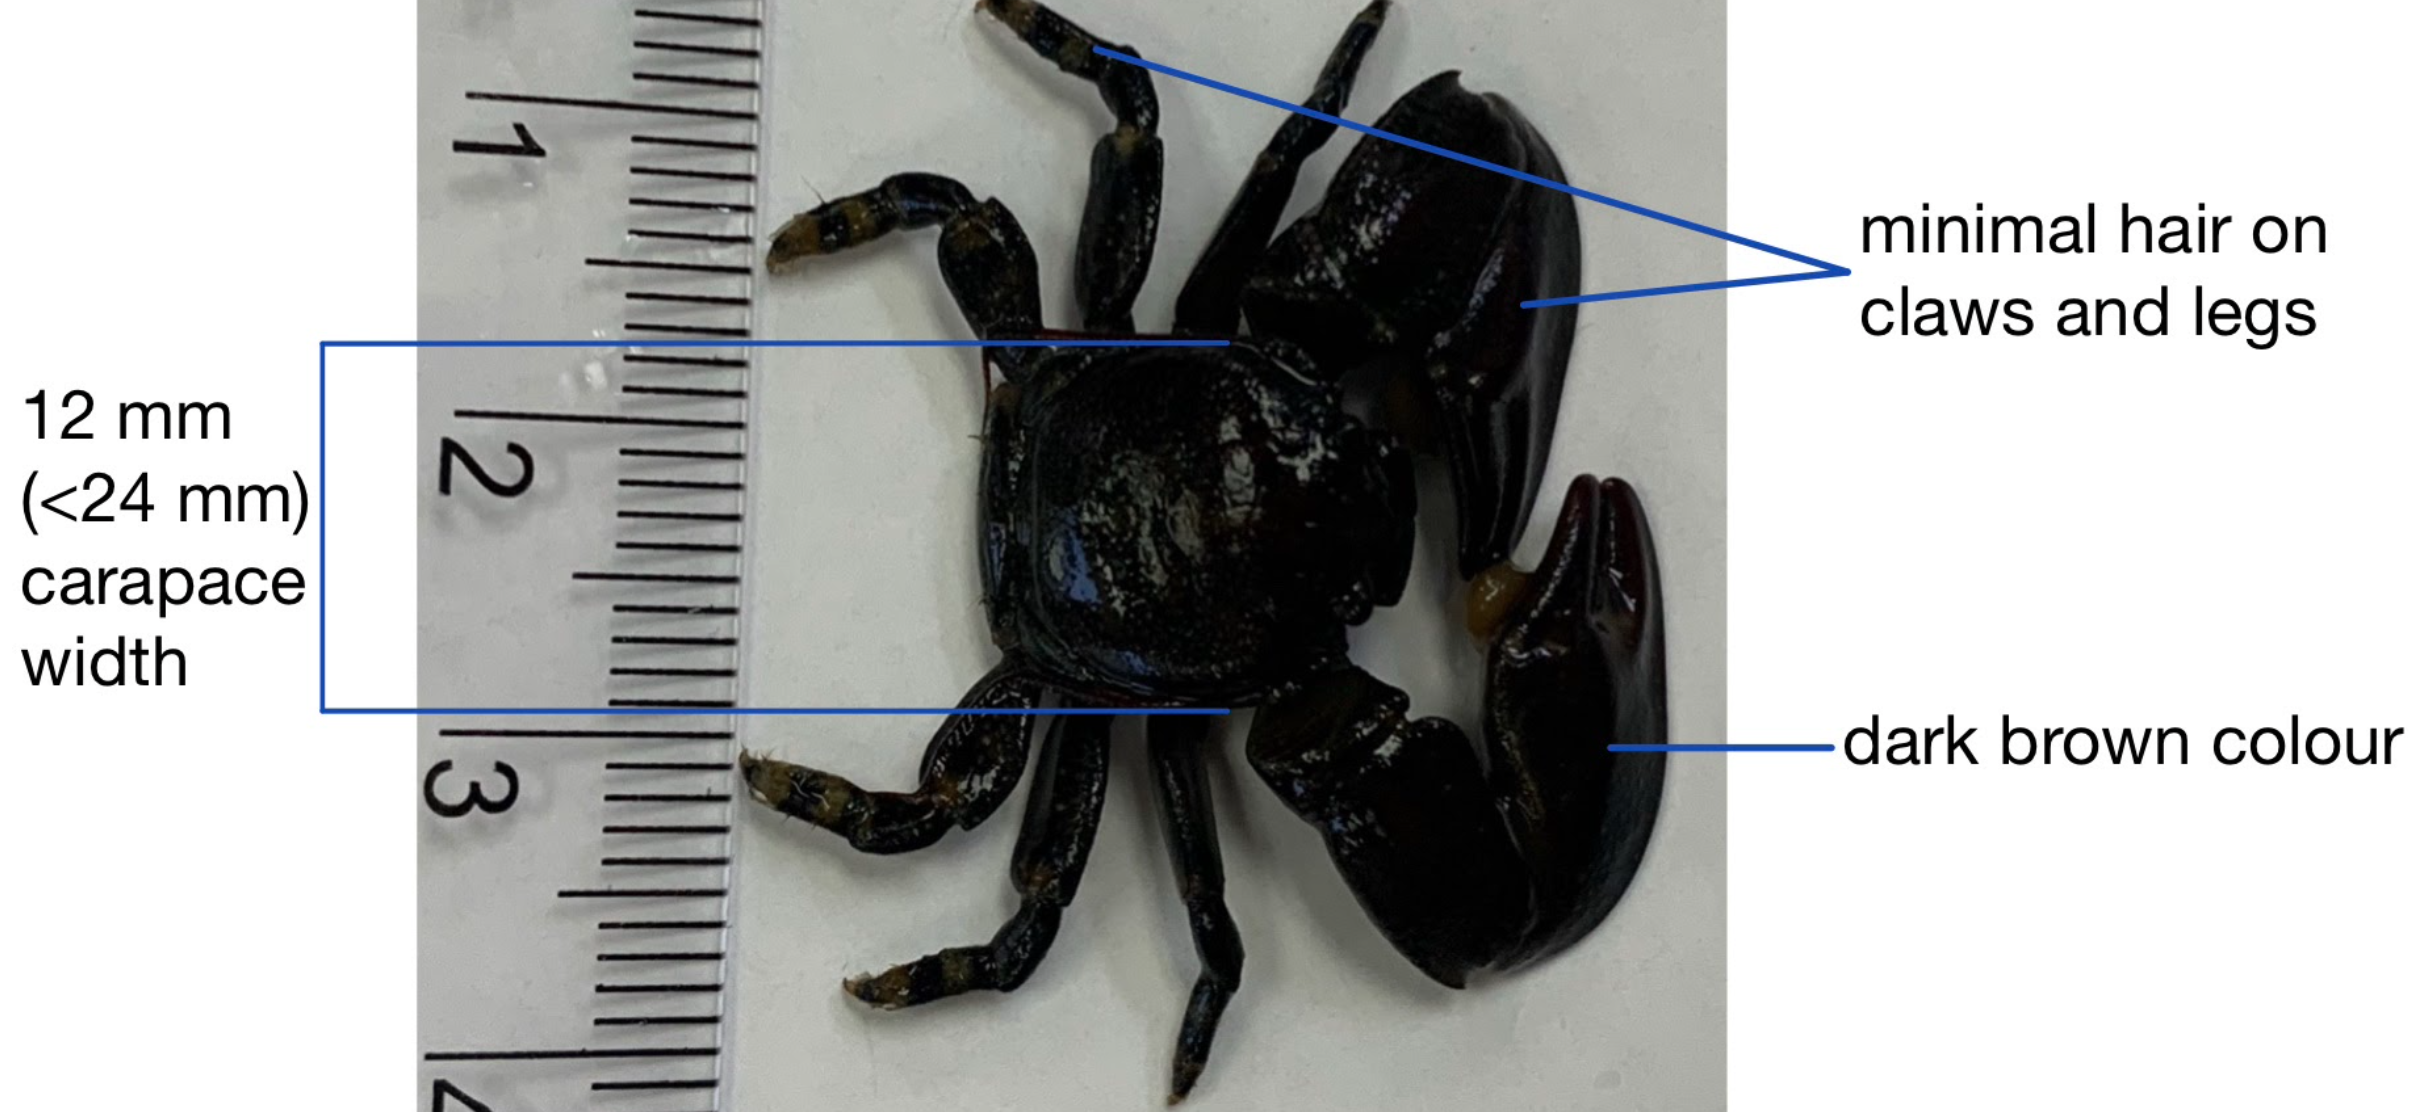
\includegraphics[width=0.5\linewidth,height=0.3\textheight]{C:/Users/bmsuser/Github/species-id-guide-genagardens/images/porcelain.carapce} \hfill{}

\caption{This is the top view of the flat porcelain crab.}\label{fig:porcelain.carapace}
\end{figure}

\begin{figure}

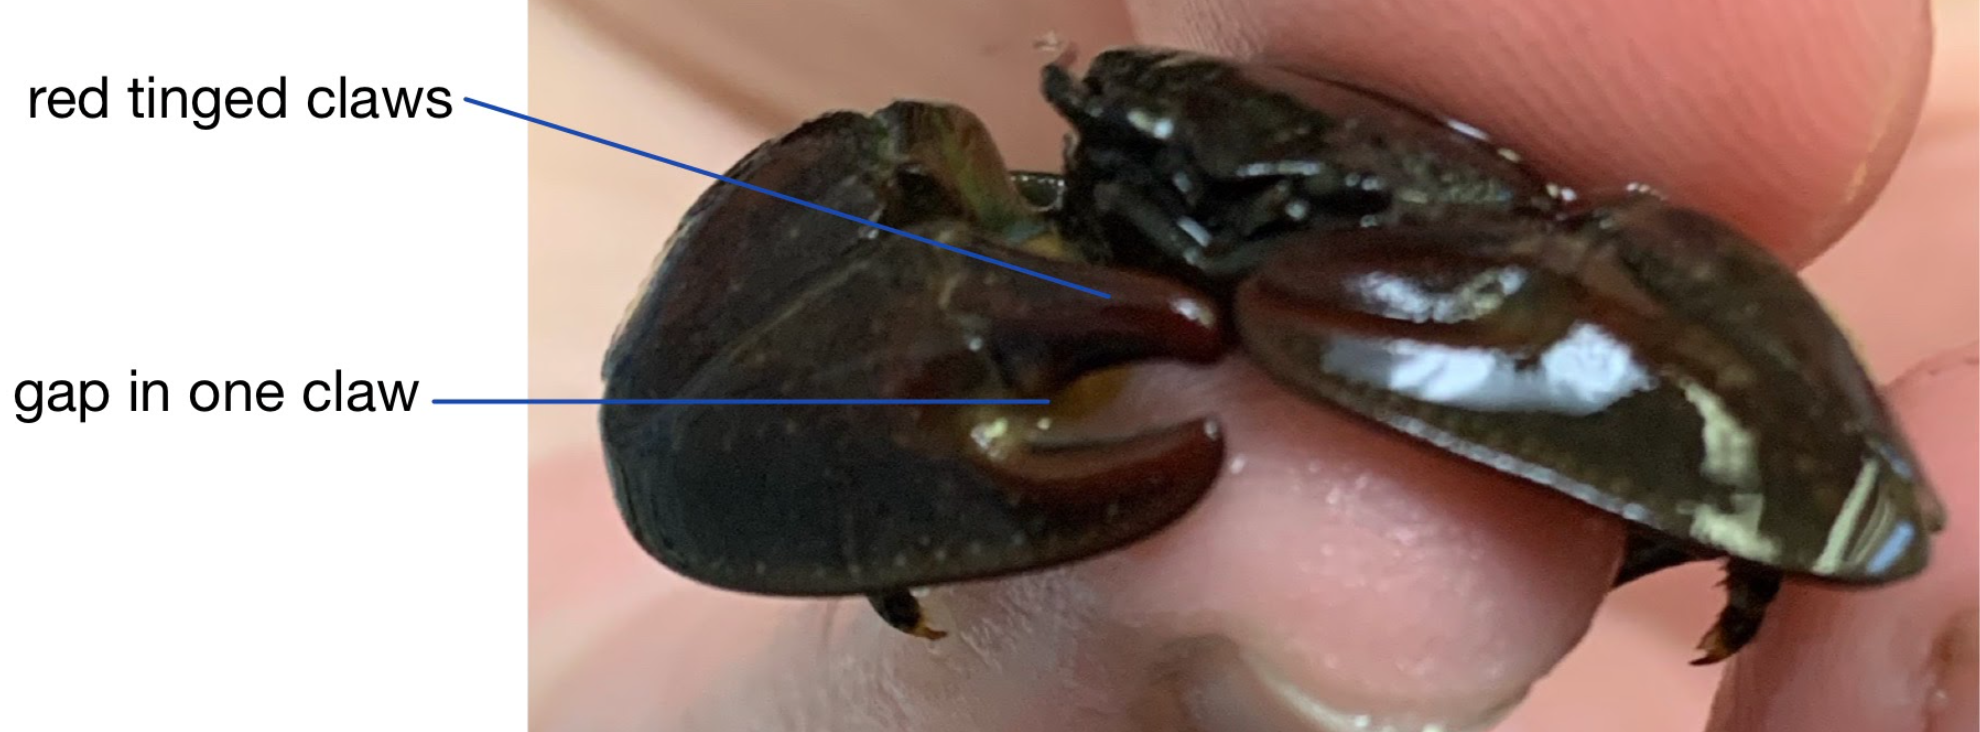
\includegraphics[width=0.5\linewidth,height=0.3\textheight]{C:/Users/bmsuser/Github/species-id-guide-genagardens/images/porcelain.claws} \hfill{}

\caption{This is the front view of the flat porcelain crab to highlight claw shape and colour.}\label{fig:porcelain.claws}
\end{figure}
\newpage

\hypertarget{questions-2}{%
\subsection{Questions}\label{questions-2}}

\begin{enumerate}
\def\labelenumi{\arabic{enumi}.}
\tightlist
\item
  Is it a small (up to 24mm in body carapace length) intertidal crab
  with obnoxiously large claws? Yes - go to question 2.\\
\item
  Is it reddish brown, dark brown or blue with distinctly red antennae?
  Yes - go to question 3.\\
\item
  Does it have distinctly hairy legs and claws? No - this is \emph{P.
  cinctipes}.
\end{enumerate}

\newpage

\hypertarget{hemigrapsus-oregonensis-hairy-shore-crab}{%
\section{\texorpdfstring{\emph{Hemigrapsus oregonensis} (Hairy shore
crab)}{Hemigrapsus oregonensis (Hairy shore crab)}}\label{hemigrapsus-oregonensis-hairy-shore-crab}}

\hypertarget{description-3}{%
\subsection{Description}\label{description-3}}

\emph{Hemigrapsus oregonensis} has 5 pairs of legs, one of which are
modified to act as claws; this is a trait of a ``true crab'' (Harbo,
2011). They have a hard top shell called a carapace that grows to a max
of 5 cm in width and displays a wide variety of colouring and patterns
(Harbo, 2011; Jensen, 1995). \emph{H. oregonensis} is morphologically
defined as having a notch between their eyes and three pairs of teeth
along the side of their carapace (Jensen, 2014) This species also has
short hairs found on the walking legs and white claws that can be used
to differentiate from other shore crabs (Jensen, 2014).

Hairy shore crabs can be dark green to grayish with some displaying
white or even purple on their square carapace (Jensen, 1995).
Polymorphism and the disruptive colouration of the morphs allow for
\emph{H. oregonensis} to camouflage within their environment by breaking
up the outline of their carapace (Jesen \& Egnotovich, 2015) Younger
individuals tend to show more variation compared to adults, and darker
morphs have the ability to alter their colouration later on in their
lifecycle (Jensen \& Egnotovich, 2015).

\textbf{Species lookalike} \emph{H. oregonensis} has similar morphology
to \emph{Hemigrapsus nudus}. \emph{H. nudus} commonly known as the
purple shore crab has purple morphs and dark spots on their modified
legs (Harbo, 2011). Compared to the \emph{H. oregonensis} the walking
legs lack the setae that give the hairy look (Harbo, 2011)

\textbf{Range, Habitat, Diet, Foraging Mode and Reproduction}\\
The \emph{H. oregonensis} is a common species that ranges from Alaska to
California baja, Mexico (Harbo, 2011). This species can be found in the
low intertidal zones on mud or sand flats (Jensen \&Egnotovich, 2015).
They tend to hide under rocks in less exposed areas (Jensen, 1995).
Hairy shore crabs were abundant on the rocky shores of Scotts bay in
Bamfield, British Columbia, where their habitat was composed of a large
variety of coloured rocks. These crabs are detritivores that consume
algae and smaller invertebrates, they also are filter feeders and act as
consumers within the food web. (Jensen, 1995). Their broad diet
classifies them as generalists, this reduces the stress on resources
within an ecosystem. As scavengers they are also important for reducing
the amount of dead organic matter that is found within the ecosystem
thus keeping it clean and non toxic for other organisms.

This species has distinct individuals that either produce female or male
gametes. They are oviparous and reproduce sexually. Research has found
that females reach sexual maturity when their carapace is 10cm in width,
but little is known about males (Jensen \& Egnotovich, 2015). Females
can produce two broods per year, each brood can contain 800 to 11,000
embryos (Strathmann, 2017).

\newpage

\hypertarget{figures-2}{%
\subsection{Figures}\label{figures-2}}

\begin{figure}

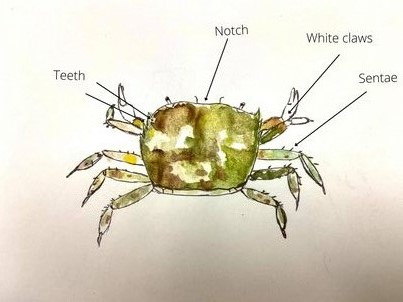
\includegraphics[width=0.5\linewidth,height=0.3\textheight]{C:/Users/bmsuser/Github/species-id-guide-genagardens/images/hairyshorecrabdiagram} \hfill{}

\caption{ Diagram of the key characteristics of $\textit{H.oregonensis}$}\label{fig:crab-water-colour}
\end{figure}

\begin{figure}

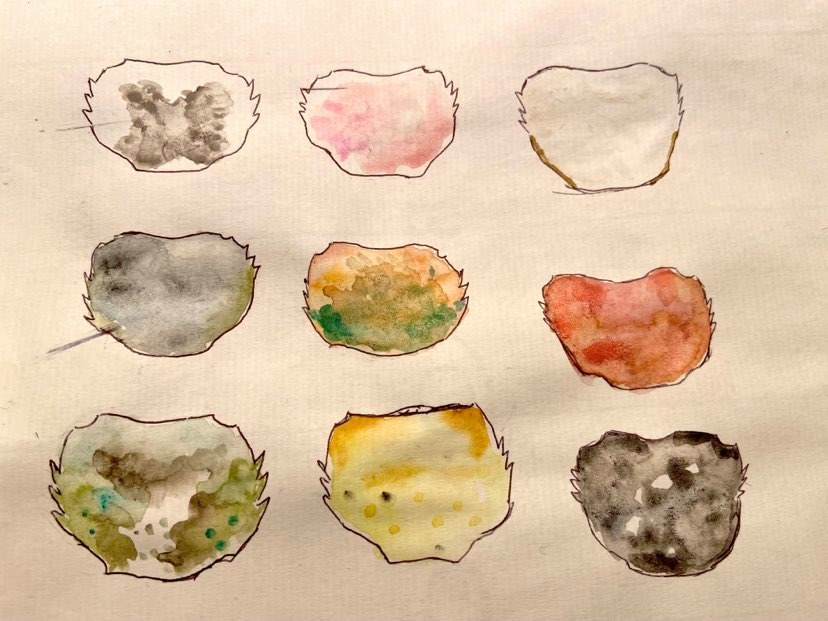
\includegraphics[width=0.5\linewidth,height=0.3\textheight]{C:/Users/bmsuser/Github/species-id-guide-genagardens/images/hairs_shore_crab_colour_variation} \hfill{}

\caption{Diagram of the hairy shore crab colour variation}\label{fig:crab-diversity}
\end{figure}

\begin{figure}

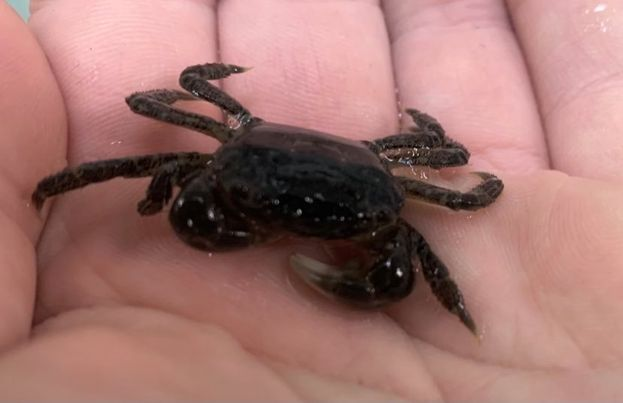
\includegraphics[width=0.5\linewidth,height=0.3\textheight]{C:/Users/bmsuser/Github/species-id-guide-genagardens/images/hairy-shore-crab} \hfill{}

\caption{Dark morph of a male hairy shore crab}\label{fig:crab-in-hand}
\end{figure}

\newpage

\hypertarget{questions-3}{%
\subsection{Questions}\label{questions-3}}

1.Does the carapace have 3 teeth?\\
2. Are the tips of the pinchers white or slightly yellow?\\
3.Does this organism have little hairs (setae) found on its legs?

\newpage

\hypertarget{references}{%
\subsection{References}\label{references}}

Cowles, D. (2005a). \emph{Pagurus granosimanus} (Stimpson, 1858).
Retrieved October 17, 2021, from
\url{https://inverts.wallawalla.edu/Arthropoda/Crustacea/Malacostraca/Eumalacostraca/Eucarida/Decapoda/Anomura/Family_Paguridae/Pagurus_granosimanus.html}.

Cowles, D. (2005b). \emph{Pagurus hirsutiusculus} (Dana, 1851).
Retrieved October 16, 2021, from
\url{https://inverts.wallawalla.edu/Arthropoda/Crustacea/Malacostraca/Eumalacostraca/Eucarida/Decapoda/Anomura/Family_Paguridae/Pagurus_hirsutiusculus.html}

Cowles, D. (2006). \emph{Petrolisthes cinctipes} (Randall, 1839).
Retrieved October 17, 2021, from
\url{https://inverts.wallawalla.edu/Arthropoda/Crustacea/Malacostraca/Eumalacostraca/Eucarida/Decapoda/Anomura/Family_Porcellanidae/Petrolisthes_cinctipes.html}

Fretwell, K. (2015). \emph{Grainyhand hermit - Pagurus granosimanus}.
Biodiversity of the Central Coast. Retrieved October 17, 2021, from
\url{https://www.centralcoastbiodiversity.org/grainyhand-hermit-bull-pagurus-granosimanus.html}.

Fretwell, K., Starzomski, B. (2014). \emph{Flat porcelain crab.}
Retrieved October 17, 2021, from
\url{https://www.centralcoastbiodiversity.org/flat-porcelain-crab-bull-petrolisthes-cinctipes.html}

Harbo, R. M. 2011. \emph{Whelks to whales}. Harbour Publishing Co.~Ltd.~

Jensen, G. C. (2014). \emph{Crabs and shrimps of the Pacific coast}.
MolaMarine.

Jensen, G. C. (1995). \emph{Pacific coast crabs and shrimps}. Sea
Challengers.\\
Jensen, G. C., \& Egnotovich, M. S. (2015). A whiter shade of male:
Color background matching as a function of size and sex in the Yellow
Shore Crab Hemigrapsus oregonensis (Dana, 1851). \emph{Current Zoology},
61(4), 729--738. \url{https://doi.org/10.1093/czoolo/61.4.729}
Kornienko, E. S. (2020). The reproductive strategy of hermit crabs in
temperate waters. \emph{Russian Journal of Marine Biology}, 46(5),
319--329. \url{https://doi.org/10.1134/S1063074020050053}

Meschkat, C., Fretwell, K., \& Starzomski, B. (2014). \emph{Hairy hermit
crab}. Retrieved October 16, 2021, from
\url{https://www.centralcoastbiodiversity.org/hairy-hermit-crab-bull-pagurus-hirsutiusculus.html}

Strathmann, M. F. (2017). \emph{Reproduction and development of marine
invertebrates of the Northern Pacific coast data and methods for the
study of eggs, embryos, and larvae.} University of Washington Press.

Yockachonis, T., McKeon, C. S., Windsor, A. M., Stillman, J. H. (2020).
Multiple paternity in the intertidal zone porcelain crab
\emph{Petrolisthes cinctipes} Randall, 1840 (Decapoda: Anomura:
Porcellanidae) is a life-history strategy that increases fitness during
heat stress. \emph{Journal of Crustacean Biology}, 40(6), 684--691.
\url{https://doi.org/10.1093/jcbiol/ruaa071}

\newpage

\hypertarget{supplemental-information}{%
\section{Supplemental Information}\label{supplemental-information}}

\begin{figure}

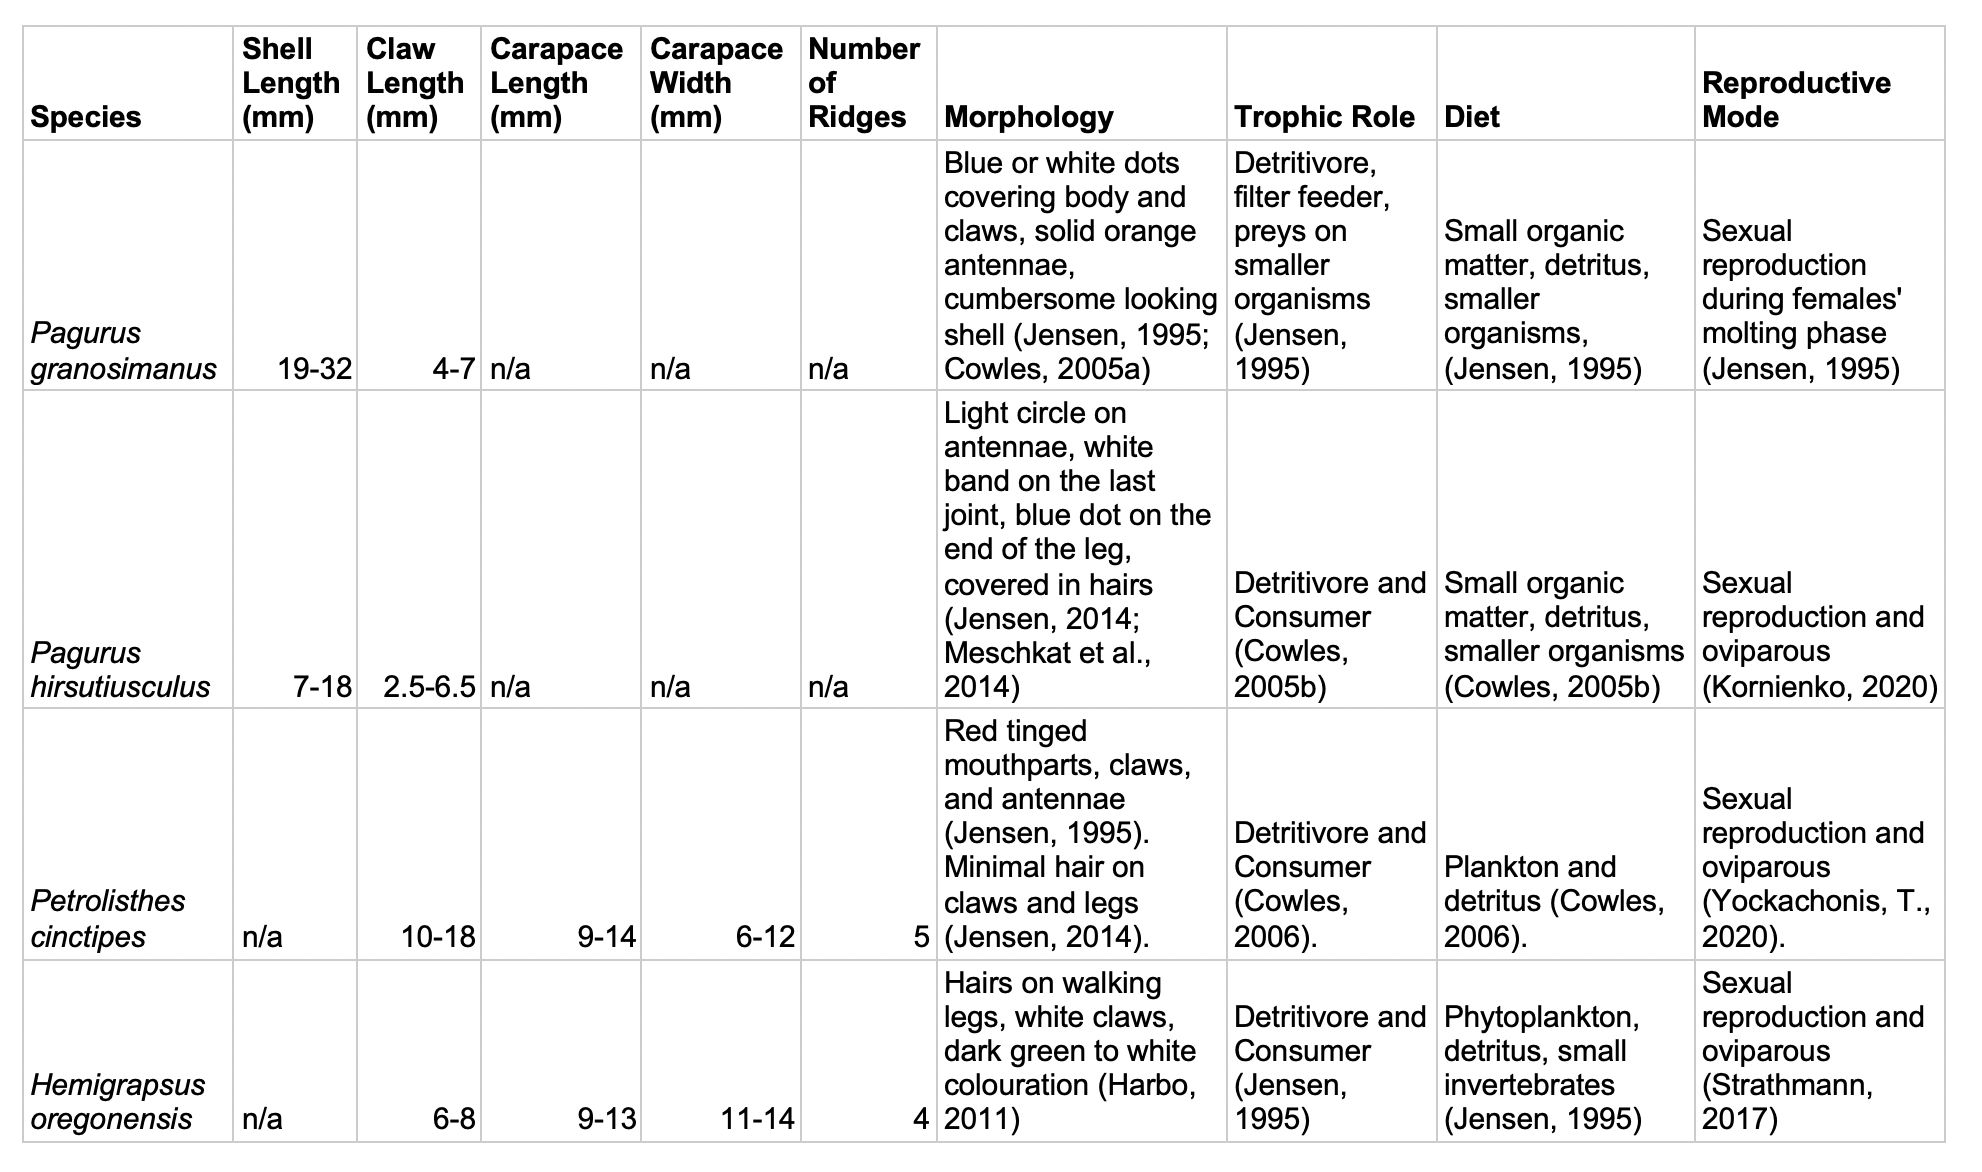
\includegraphics[width=0.9\linewidth,height=0.8\textheight]{C:/Users/bmsuser/Github/species-id-guide-genagardens/images/summary-table} \hfill{}

\caption{Table 1: A summary of measurements collected in field, morphology, trophic role, diet and reproduction for the four species of crabs}\label{fig:summary-table}
\end{figure}

\hypertarget{figures-3}{%
\subsection{Figures}\label{figures-3}}

\begin{figure}
\includegraphics[width=0.5\linewidth,height=0.5\textheight]{species-id-guide-desjardin_files/figure-latex/unnamed-chunk-2-1} \caption{Shell length and claw length compared by species in hermit crabs.}\label{fig:unnamed-chunk-2}
\end{figure}

\begin{figure}
\includegraphics[width=0.5\linewidth,height=0.5\textheight]{species-id-guide-desjardin_files/figure-latex/unnamed-chunk-3-1} \caption{Carapace length and width compared by species of shore crabs.}\label{fig:unnamed-chunk-3}
\end{figure}

\begin{figure}
\includegraphics[width=0.5\linewidth,height=0.5\textheight]{species-id-guide-desjardin_files/figure-latex/unnamed-chunk-4-1} \caption{Number of spines and claw length compared by species of shore crabs.}\label{fig:unnamed-chunk-4}
\end{figure}

\end{document}
